%% -*- TeX-engine: luatex; ispell-dictionary: "russian" -*-

\documentclass[a4paper,12pt]{article}

\usepackage[left=1.5cm,right=2cm,top=1.5cm,bottom=2cm]{geometry}

\usepackage{parskip}
\setlength{\parindent}{0mm}
\setcounter{secnumdepth}{1}

\usepackage{amsmath}

\usepackage{graphicx}

\usepackage{fontspec}
\setmainfont{PT Serif}
\newfontfamily\cyrillicfont[Script=Cyrillic,Ligatures=TeX]{PT Serif}
\setsansfont{PT Sans}
\setmonofont[Ligatures=NoCommon]{PT Mono}
\defaultfontfeatures{Ligatures=TeX}

\usepackage[bold-style=ISO]{unicode-math}
\setmathfont{XITS Math}

\usepackage{microtype}

\usepackage{hyperref}

\usepackage{polyglossia}
\setmainlanguage{russian}
\setotherlanguage{english}

\usepackage{csquotes}

%% for code snippets
\usepackage{minted}
\newminted[pycon]{pycon}{fontsize=\footnotesize}
\newminted[python3]{python3}{fontsize=\footnotesize}
\newminted[bash]{bash}{fontsize=\footnotesize}
\newmintinline[pythoninline]{python3}{fontsize=\footnotesize}
\newmintinline[bashinline]{bash}{fontsize=\footnotesize}

\pagestyle{empty}


\begin{document}
\subsection*{Домашнее задание №5: <<Индейцы пима, диабет и линейный классификатор>>}

\begin{tabular}{@{}lr}
  \textbf{Дедлайн 1} (20 баллов): & 2 апреля, 23:59 \\
  \textbf{Дедлайн 2} (10 баллов): & 9 апреля, 23:59 \\
\end{tabular}

Домашнее задание нужно написать на Python и сдать в виде одного файла.
Правило именования файла: \texttt{name\_surname\_5.[py | ipnb]}. Например, если
вас зовут Иван Петров, то имя файла должно быть: \texttt{ivan\_petrov\_5.py} или \texttt{ivan\_petrov\_5.ipnb}.

\makebox[\linewidth]{\hrulefill}

\begin{figure}[h!]
  \centering
  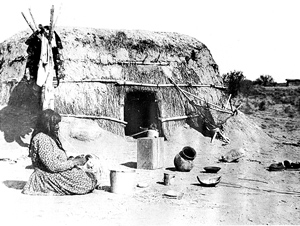
\includegraphics[width=.4\linewidth]{images/pima}
  \caption{Источник: \url{http://gilariver.org}}
\end{figure}

Индейцы племени пима проживают в центральной и южной части штата Аризона. По
неизвестным на данный момент причинам индейцы пима имеют критический риск
заболевания сахарным диабетом (2 типа). В этом задании предлагается применить
линейный классификатор для диагностики и изучения сахарного диабета (2 типа) у
представителей племени пима.

По ссылке%
\footnote{\url{https://gist.github.com/ktisha/c21e73a1bd1700294ef790c56c8aec1f}}
находятся медицинские данные представителей племени пима. Последняя колонка
каждой строки --- индикатор наличия сахарного диабета (2 типа). Значения
остальных колонок указаны в заголовке файла.

\pagebreak

\paragraph{1} Реализуйте функцию \pythoninline{read_data}, которая принимает
путь к файлу с данными и возвращает пару из двух массивов NumPy\footnote{Хорошее
  введение в API массивов NumPy можно найти на сайте
  \url{http://scipy-lectures.github.io/intro/numpy}}.
\begin{itemize}
\item Первый элемент пары --- матрица признаков \pythoninline{X}, в первой
  колонке которой находится константный признак -1, а в остальных признаки из
  файла с данными.
\item Второй элемент пары --- вектор \pythoninline{y}, в котором -1 означает
  наличие диабета, а 1 --- его отсутствие.
\end{itemize}

Возможно, вам будет полезна функция \pythoninline{genfromtext}, читающая матрицу
NumPy из CSV файла.

\paragraph{2} Реализуйте несколько вариантов функции потерь. Функция потерь
должна принимать на вход \textbf{вектор} отступов \pythoninline{M} и возвращать
пару из вектора значений функции потерь и вектора её производных. Например, если
бы мы решили использовать степенную функцию потерь:
\begin{python3}
def power_loss(M, n=5):
    return M ** (-n), -n * (M ** (-n - 1))
\end{python3}

Необходимо реализовать как минимум логарифмическую (\pythoninline{log_loss}) и
сигмоидную (\pythoninline{sigmoid_loss}) функции потерь.

\paragraph{3} Реализуйте метод градиентного спуска для обучения линейного
классификатора в виде класса \pythoninline{GradientDescent}. Структура класса
приведена ниже:
\begin{python3}
class GradientDescent:
    def __init__(self, *, alpha, threshold=1e-2, loss=sigmoid_loss):
        if alpha <= 0:
            raise ValueError("alpha should be positive")
        if threshold <= 0:
            raise ValueError("threshold should be positive")
        self.alpha = alpha
        self.threshold = threshold
        self.loss = loss

    def fit(self, X, y):
        errors = []
        # ...
        return errors

    def predict(self, X):
        # ...
\end{python3}

Метод \pythoninline{fit} должен:
\begin{itemize}
\item случайно инициализировать веса,
\item оценить веса линейного классификатора с использованием функции потерь,
\item записать полученные веса в атрибут \pythoninline{self.weights}
\item и вернуть список значений функционала качества $Q(\mathbf{w})$ на
  каждой итерации градиентного спуска.
\end{itemize}

Результатом метода \pythoninline{predict} является вектор предсказаний из -1 и 1,
полученный с использованием весов, оцененных в методе \pythoninline{fit}.

В качестве критерия остановки следует использовать отсечку
\pythoninline{threshold} на расстояние между векторами весов на текущей и
предыдущей итерациях. Расстояние можно выбрать любое, например, Евклидово или
$\ell^1$.

Обратите внимание, что на данных индейцев пима алгоритм должен работать
\textbf{не более} 30 секунд.

\paragraph{4} Реализуйте метод стохастического градиентного спуска для обучения
линейного классификатора. Структура класса аналогична:
\begin{python3}
class SGD:
    def __init__(self, *, alpha, loss=log_loss, k=1, n_iter=100):
        if alpha <= 0:
            raise ValueError("alpha should be positive")
        if k <= 0 or not isinstance(k, int):
            raise ValueError("k should be a positive integer")
        if n_iter <= 0 or not isinstance(n_iter, int):
            raise ValueError("n_iter should be a positive integer")

        self.k = k
        self.n_iter = n_iter
        self.alpha = alpha
        self.loss = loss

    def fit(self, X, y):
        errors = []
        # ...
        return errors

    def predict(self, X):
        # ...
\end{python3}

Как и в случае с \pythoninline{GradientDescent} метод \pythoninline{fit} должен
возвращать значения $Q$ на каждой итерации. Значение $\eta \in [0, 1]$,
используемое для вычисления оценки $Q$, можно выбрать любое, например,
\pythoninline{1 / len(X)}. Так как величина $Q$ не стабильна, использовать
её для определения сходимости не следует. Вместо этого предлагается
использовать ``стратегию оптимиста'': сделать ровно \pythoninline{n_iter}
итераций и надеяться, что за это время стохастический градиентный спуск
сойдётся.

Параметр \pythoninline{k} определяет размер случайной подвыборки из
\pythoninline{X}, используемой для вычисления градиента. Такой вариант
стохастического градиентного спуска называется \emph{mini-batch}. При
\pythoninline{k = 1} он вырождается в алгоритм, описанный на лекции.

Обратите внимание, что на данных индейцев пима 1000 итераций алгоритма должна
занимать \textbf{не более} 30 секунд.

\paragraph{5} Воспользуйтесь функциями \pythoninline{test_train_split} и
\pythoninline{print_precision_recall} из домашнего задания 2 для оценки качества
работы реализованных алгоритмов на данных индейцев пима.

\paragraph{6} Исследуйте чувствительность алгоритмов к выбору параметров.

\begin{itemize}
\item Постройте график функционала качества $Q(\mathbf{w})$ алгоритма
  \pythoninline{GradientDescent} в зависимости от значения $\alpha \in
  \{10^{-6}, 10^{-4}, 10^{-2}, 1\}$.
\item Постройте аналогичный график для оценки значения функционала качества $Q$
  алгоритма \pythoninline{SGD} в зависимости от $\alpha$ и $k \in \{1, 10,
  50\}$.
\end{itemize}

Графики необходимо построить для всех реализованных вами функций потерь и
приложить к письму.

\paragraph{7} Ответьте на вопросы с использованием графиков.
\begin{itemize}
\item Почему функционал качества убывает в процессе работы градиентного
  спуска? Почему это не всегда так для стохастического градиентного спуска?
\item Как зависит скорость сходимости (количество итераций) алгоритмов от $\alpha$?
\item Как параметр $k$ влияет на поведение $Q$ в алгоритме стохастического
  градиентного спуска?
\item Какие значения параметров каждого алгоритма вам кажутся оптимальными для
  задачи диагностики диабета? Почему?
\item Как ведёт себя вектор весов $\mathbf{w}$ при повторных запусках
  алгоритмов? Объясните причины наблюдаемого поведения.
\item Какой алгоритм уместнее использовать для данных индейцев пима? Почему?
\end{itemize}

\paragraph{8} Приведите наиболее симпатичный вам вектор весов $\mathbf{w}$ и
дайте интерпретацию его значениями применительно к задаче диагностики диабета
или объясните, почему это невозможно.

\end{document}
